\documentclass[11pt]{article}
\usepackage[letterpaper]{geometry}
\usepackage{microtype}
\usepackage{url}
\usepackage{setspace}
\usepackage{enumitem}
\usepackage{amsmath}
\usepackage{graphicx}
\usepackage{color}
\usepackage[dvipsnames]{xcolor}
\usepackage{soul}
\usepackage{hyperref}
\hypersetup{hidelinks}
\usepackage[numbers,sort&compress]{natbib}

% Hogg issues
\setlength{\topmargin}{0in}
\setlength{\headsep}{0in}
\setlength{\headheight}{0in}
\setlength{\oddsidemargin}{0in}
\setlength{\textheight}{9in}
\setlength{\textwidth}{6.5in}
\sloppy\sloppypar\raggedbottom\frenchspacing
\setstretch{1.08} % 
\renewcommand{\Large}{\normalsize} 
\renewcommand{\large}{\normalsize} 
\renewcommand{\paragraph}[1]{\medskip\par\noindent\textbf{#1~---}}
\setlist{topsep=0.75ex, itemsep=0.75ex, parsep=0ex} % This tightens up ALL lists.

\newcommand{\kw}[1]{{\color{RoyalBlue}[KW: #1 ]}}
\newcommand{\hogg}[1]{{\color{red}[Hogg say: #1 ]}}
\newcommand{\remove}[1]{{\color{red}\st{#1}}}
\frenchspacing


%TODO
%HOGG: put words on bias-variance

\begin{document}

\section*{Cover Page}

\clearpage
\renewcommand{\contentsname}{Table of Contents}
\tableofcontents

\bigskip
\noindent{~\hfill --------- \hfill~}
\bigskip

\section{Technical Approach}
\subsection*{\raggedright Mathematically principled machine learning approaches to ocean dynamics}

The theory of the oceans and the atmosphere is, fundamentally, a computational theory, which requires simulations to solve and understand their complex evolution.
These simulations are extremely expensive multi-physics, multi-scale computations, and yet they don't currently have anything like the resolution they would need to resolve all scales of physical interest.
At the same time, making predictions for weather and climate depends on being able to run very large numbers of these simulations, both to match the data in the sense of a digital twin for the Earth, and also to quantify uncertainties.

For all these reasons, the ocean dynamics community has been looking at machine learning (ML) approaches.
Emulators---ML regressions trained on good, first-principles, physics simulations---can predict the outcomes of physics simulations with far less computation than that used by the simulations on which they are trained.
Also, sub-grid models built out of ML components can be trained to predict the differences between low-resolution and high-resolution simulations, which arise from non-linear dynamics.
These can be used to either speed high-resolution simulations (by patching low-resolution simulations), or else to make predictions for small scales that aren't even resolved with the highest resolution simulations (that is, provide closure).

Generalizing beyond Earth science, there is a growing interest in replacing or augmenting solvers for partial differential equations (PDEs) with ML regressions trained on computed data.
These projects have applications across many physics and engineering domains.
Since PDEs are the underlying technology in simulations of physical systems at many scales from electronics to the entire visible Universe,
these approaches to speeding up PDEs will speed up any kinds of digital twins---virtual representations of objects or systems (in this case the ocean)---designed to reflect particular physical objects accurately.

Recent applications of emulation in ocean dynamics contexts have shown some important successes, for example
an idealized model for multi-decadal timescales based on neural operators \cite{bire2023ocean}, a regional emulation on subseasonal timescales 
\cite{chattopadhyay2023oceannet}, and a 3D global emulation on 30-day timescales
\cite{xiong2023ai}.
Recent work by PI Zanna builds ML-based ocean emulators for multi-century rollouts that incorporate atmospheric data~\cite{subel2024building, thermalizer}. 

These ML approaches are very promising; they are driving innovation and research in ocean science and PDEs.
Because of the immense computational speed-ups that they enable, they are making possible computational programs that weren't previously possible.
At the same time, PIs Hogg and Villar have warned that the introduction of ML in these contexts can lead to important statistical biases \cite{goodorbad}.
The important question is: How can we trust and verify predictions made by ML models trained on simulations?
A hallmark of contemporary ML methods---such as convolutional neural networks, and transformers---is that they are enormously over-parameterized, contain internal combinatorially large degeneracies, and are essentially impossible to interpret at the parameter level.
In addition and relatedly, ML models are generically subject to successful adversarial attacks.
These attacks are often very highly tuned, specific problems with specific trained models.
But they reveal that the ML models are not doing what we expect, and that they are uninterpretable, and (in some sense) untrustworthy.

The trustworthiness issue originates from the fact that the accuracy of a ML solution does not have guarantees at run time, which is particularly important when ML is being applied to problems that have inherently low risk tolerance, such as medical operations, self-driving cars, and studies of global climate.
The possibility of potential catastrophic failures casts doubt on adopting ML solutions at scale, especially in the domains of greatest interest to agencies (such as ONR) and researchers.
Thus some of the research proposed here has implications that go far beyond PDEs.

The question in this proposal is:
How can we make ML methods used to emulate or improve numerical solutions to PDEs---and in particular, in ocean dynamics---more trustworthy?
We will explore answers to this question in part by implementing exact symmetries and by forcing latent models to obey exact, local conservation laws (allowing for the fact that real data sets often break these symmetries), and in part by developing adversarial training strategies.
In this work, we are building on our research in mathematical machine learning, in which we have shown that making ML methods obey the exact symmetries of classical physics improves prediction accuracy for physics problems, permits out-of-sample generalization, and reduces training-set data requirements.
Here we propose to extend this work to ocean contexts, and to the specific cases of closure of PDEs and emulation.
And we propose to empirically test our successes with uncertainty quantification and adversarial attacks.
This project will produce scientific papers; it will produce robust code to emulate simulations, quantify uncertainties, and adversarially attack; and it will produce data in the form of emulated ocean dynamics simulation outputs.
% HOGG: DO WE EXPLICITLY PROMISE TO MAKE DATA, BELOW? 

\subsection{Thrust 1: Learning ocean dynamics with the exact symmetries of classical physics}

In this project, our aim is to use the power of ML to obtain fast and robust predictions of ocean dynamics, and to understand the mathematical properties of the proposed models. In this task, we focus on defining the ML models. We consider three settings (1) the more theoretical setting in which one needs to emulate the dynamics of a known partial differential equation and/or closures need to be resolved, (2) the more practical setting in which the governing equation of the dynamics is not known but a time series of observations are provided, and (3) a hybrid setting in which data (observations) are combined with parametric partial differential equations.

What makes our approach different from others bringing ML approaches to ocean dynamics is that the models we propose here will be consistent with some of the symmetries of classical physics, which include the coordinate freedoms of rotation and translation, and the corresponding conservation laws.
Our preliminary results show that incorporating these constraints improves the robustness and generalization of the models. In the subsequent tasks we propose to empirically and mathematically evaluate these claims.

\paragraph{The closure problem}
In high-dimensional dynamical systems such as turbulent fluid dynamics and astrophysical plasmas, the physical process occurs on a wide range of spatio-temporal scales, and often processes on different scales will have their effect cascade to other scales. 
Therefore, in the ideal scenario, it is important to model all scales at the same time.
However, the computational cost usually increases geometrically with resolution, rapidly making good simulations prohibitively expensive.
For this reason, simulations are usually truncated at some scale.
This truncation inevitably loses small-scale information necessary to obtain accurate results, including even on much larger scales, because of these cascading effects.
The closure problem consists of building an effective model for the influence of the discarded degrees of freedom for all of the dynamics.

Solving the closure problem involves building and incorporating a subgrid model to compensate for missing modes.
Traditionally, there have been many attempts to use heuristic or empirical physical arguments to capture the effects of small and ``meso'' scales in the resolved flows \cite{thuburn2014cascades,jansen2014parameterizing, mana2014toward, zanna2017scale, bachman2017scale, pearson2017evaluation, bachman2018relationship, jansen2019toward, bachman2019gm, grooms2015numerical, berloff2018dynamically, juricke2020ocean}.
These models are often physically motivated and interpretable.
In recent years, ML methods have demonstrated promising results in capturing the subgrid physics with parameterized models with many parameters \cite{rasp2018deep, Bolton2019,maulik2019subgrid, beck2019deep, yuval2020stable, guan2022stable, beucler2021climate, shamekh2022implicit, wang2022non}.
Compared to physically-motivated models, ML methods have the advantage of flexibility to match complex functions.
However, this often comes at a cost of interpretability and controllability.

In particular, work by Bolton and Zanna \cite{Bolton2019} uses ML to learn forces that can correct the difference between the high-resolution model and the low-resolution model obtained after coarse-graining. These ML models are good at predicting the subgrid forcing, but they have poor performance when integrated over long periods of time. One hypothesis for this failure mode is the learned model does not respect some fundamental symmetries in the underlying physical system.

In this Thrust, we will develop equivariant ML models (i.e., ML models that are designed to respect symmetries) to learn the dynamics of an ocean model in order to understand whether adding symmetries to our model will improve its long-term stability.
We remark that some of the existing ML approaches do account for energy constraints \cite{guan2023learning} and physical invariances \cite{frezat2021physical, guan2023learning, pawar2023frame, Bolton2019} in general scenarios. Our goal is to further extend these ideas to incorporate other forms of coordinate freedom, specifically targeting oceanic dynamics. We propose to adapt the techniques from \cite{villar2021scalars} and \cite{xu2022pde} to implement a symmetry-preserving ML model for the 2-layer quasi-geostrophic (QG) ocean model implemented in \cite{pyqg}. We conjecture that incorporating symmetries and coordinate freedoms arising from physical law will improve the performance of the ML models, especially in terms of the long-term stability of the simulations.

Following \cite{pyqg}, the two-layer QG equations in Cartesian coordinates are
\begin{align} \label{eq.QG1}
    \partial_t q_m + \nabla\cdot (\mathbf u_m \,q_m) + \beta_m\, \partial_x \psi_m + U_m\,\partial_x q_m = -\delta_{m,2}\,r_{ek}\,\nabla^2\psi_m +ssd\circ q_m \\
    q_m = \nabla^2\psi_m+(-1)^m\frac{f_0^2}{g'\,H_m}(\psi_1-\psi_2), \quad m\in\{1,2\}
    \label{eq.QG2}
\end{align}
where $x$ is the zonal coordinate (east-west) and y is the meridional coordinate (north-south); $m$ is the index of the fluid layer (1 for the upper layer and 2 for the lower layer); $q_m$ is a pseudo-scalar which represents the potential vorticity (it is invariant under rotations and it changes sign under reflections); $\psi_m$ is a pseudo-scalar known as the streamfunction, which allows us to compute the (vector) velocity as 
$\mathbf u_m=(u_m, v_m) = (-\partial_y\psi_m, \partial_x \psi_m)$; $U_m$ is the prescribed mean zonal flow (in the $x$ direction); $\beta_m = \beta + (-1)^{m+1} \frac{f_0^2}{g'H_m}(U_1-U_2)$ is the meridional gradient of potential vorticity due to differential rotation and prescribed mean flow; $r_{ek}$ is the bottom drag coefficient with the ocean floor (a scalar); $\delta_{m,2}$ is a Kronecker delta that we use to indicate that this term only shows up for the lower layer; $f_0$ is the reference Coriolis frequency (a scalar); $g'$ is the reduced gravity (also a scalar); $H_m$ is the fluid layer thickness; $\nabla = (\delta_x, \delta_y)$ is the horizontal gradient operator; $ssd$ is a small-scale dissipation function from the numerical scheme (see \cite{perezhogin2023generative}, Appendix A). 

The large eddy simulation approach from \cite{sagaut2005large} decomposes the variables $\mathbf u, q, \psi$ into the sum of resolved variables $\bar{\mathbf u}, \bar q, \bar \psi$ and subgrid components  $\mathbf u', q', \psi'$. The resolved variables correspond to the coarser observations of the original variables (namely, the convolution of the original variables with a Gaussian filter or similar), and the subgrid components are unknown. 

The governing equations for the filtered solutions are:
\begin{align}
    \partial_t \bar q_m + \nabla\cdot (\bar{\mathbf u}_m\,\bar q_m) + \beta_m\,\partial_x \bar \psi_m + U_m\,\partial_x \bar q_m = -\delta_{m,2}\,r_{ek}\,\nabla^2\bar \psi_m + S_m +ssd\circ \bar q_m \\
    \bar q_m = \nabla^2\bar\psi_m+(-1)^m\frac{f_0^2}{g'\,H_m}(\bar \psi_1-\bar \psi_2), \quad m\in\{1,2\},
\end{align}
where $S_m$ is the additional (scalar) subgrid forcing produced by the unresolved eddies on the resolved scales:
\begin{equation}
    S_m = \nabla \cdot (\bar{\mathbf u}_m\,\bar q_m - \overline{\mathbf u_m\,q_m})
\end{equation}

The closure problem amounts to modeling $S_m$ such that the integration of the filtered solution in a coarse simulation matches the filtration of the solution of a higher-resolution simulation. In \cite{perezhogin2023generative} PI Zanna and collaborators use ML models to learn $S_m$ from simulated data at different resolutions. 

We propose that incorporating symmetries in the learning of the subgrid forcing will improve the learning by reducing the sample complexity and generalization error. In order to incorporate the symmetries we propose to use invariant-scalar-based models similar to the ones proposed by PIs Villar and Hogg \cite{villar2021scalars}. Similar ideas have already been applied to learning closures on different fluid dynamics PDEs in \cite{xu2022pde}.

In a nutshell, the idea is to parameterize $S_m$ as the divergence or a learned vector (or pseudo-vector) field. The vector field is parameterized as an $O(d)$-equivariant vector function with input vectors $v_1,\ldots, v_n$ and scalars $s_1,\ldots, s_k$ can be written as 
$$f(v_1,\ldots, v_n, s_1,\ldots, s_k) = \sum_{t=1}^n f_t([v_i^\top v_j]_{1\leq i \leq j \leq n },\ s_1, \ldots, s_k)v_t.$$
It may be needed to generalize this model to incorporate pseudo-vector and pseudo-scalar inputs and outputs. See \cite{gregory2023geometricimagenet} for a potential approach.

In this subtask we propose to:
(1) design an equivariant ML model to learn closures using techniques from \cite{villar2021scalars, xu2022pde}, (2) design a set of experiments to empirically assess the performance of the equivariant models in comparison with baseline ML models, (3) apply these ideas to simulated data from the ocean model QG equation, (4) provide a robust software package to reproduce these experiments and that can be extended to other equations.
See Section \ref{sec:deliverables} for more details on the deliverables on work plans. 

%This Thrust aims to improve oceanic simulations in two parallel direction: building ML-enhanced simulations and end-to-end emulation of simulations. On one hand, we will create end-to-end ML emulator to reduce the computational cost of creating large scale simulations. On the other hand, we will apply ML methods to replace uncertain terms in QG models in order to improve accuracy of existing model; 

\begin{figure}
    \centering
    \begin{minipage}{0.37\textwidth}
    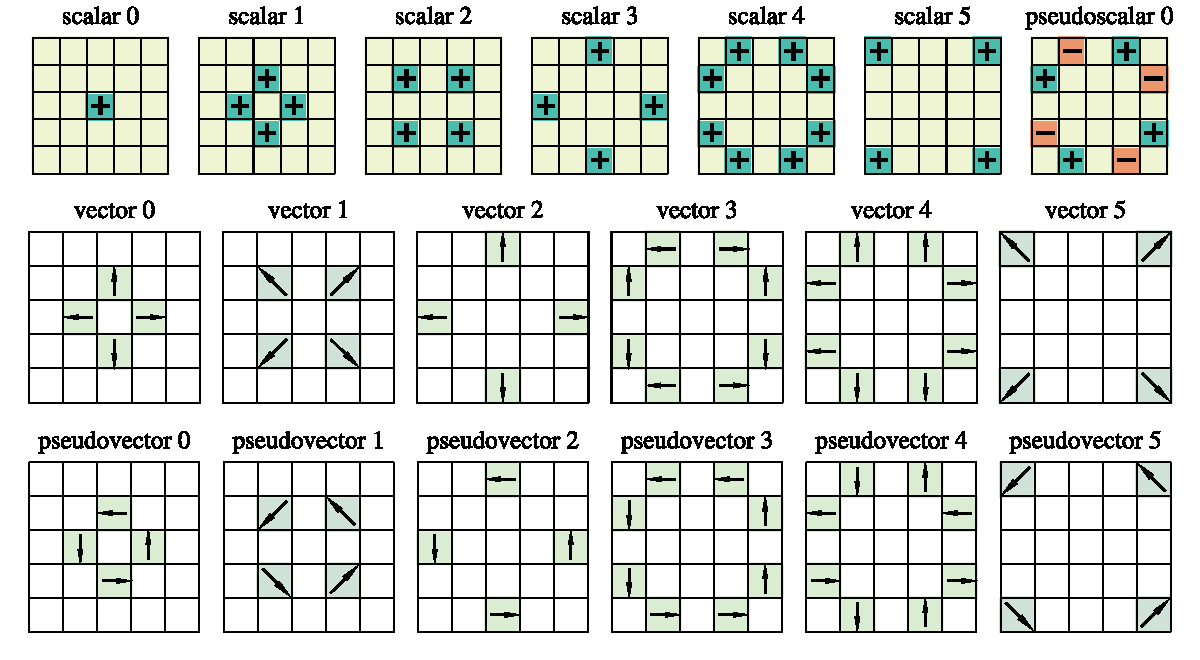
\includegraphics[width=\textwidth]{figures/filters_m5.pdf}
    \end{minipage}
    \begin{minipage}{0.62\textwidth}
    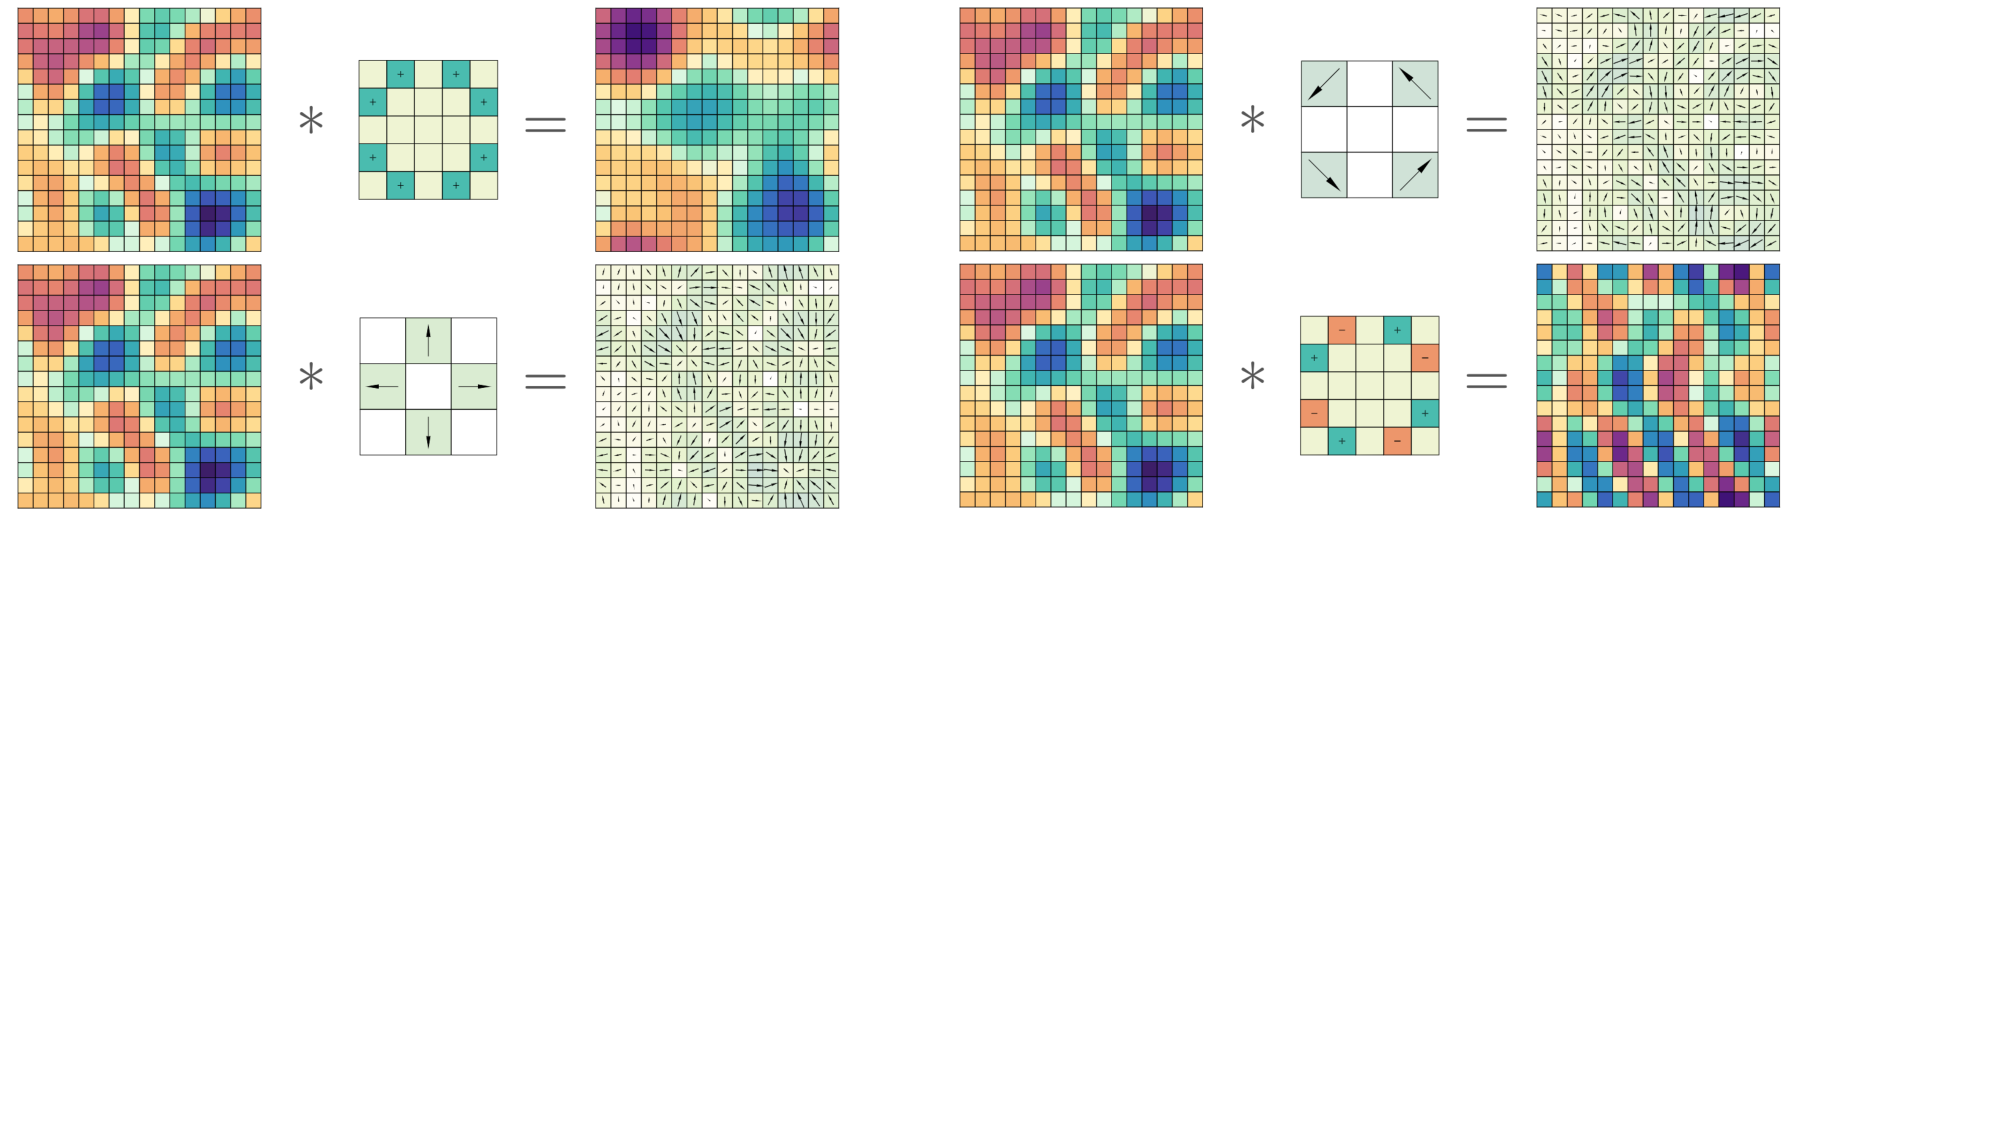
\includegraphics[width=\textwidth]{figures/convs.pdf}
    \end{minipage}
    \caption{(Left) The 5x5 scalar, pseudoscalar, vector, and pseudovector symmetric filters of GeometricImageNet for 2-D images. (Right) Convolution of a scalar image with different geometric filters. Note the convolution with a scalar filter can be seen as the discretization of a diffusion operator, and the convolution with the vector filter resembles a discretization of the gradient. In general any symmetric discretization of any coordinate-free operator (gradient, divergence, curl) could be expressed in terms of our symmetric filters.}
    \label{fig.GINet}
\end{figure}

\paragraph{End-to-end emulation of simulations}
Ocean dynamics involves processes at many different scales. This means a detailed ocean simulation requires resolving small-scale processes over a large volume, which demands significant computational power.
Instead of solving the dynamic equations from first principles, a promising and increasingly popular way to amortize the computational cost is to train a ML model over a set of training simulations. Once the ML model is trained, one can use it to generalize to settings where the model is not trained. This method has shown promising results in a number of multiscale problems, including weather forecasting \cite{Pathak2022FourCastNetAG} and cosmological simulations \cite{CAMELS:2020cof}. However, existing methods often employ ML methods that do not explicitly preserve symmetries in the simulations, which could lead to potential inaccuracy. The goal of this task is to investigate whether equivariant ML models can outperform non-equivariant models for ocean modeling.

In \cite{Gregory2023EquivariantGC} we introduced GeometricImageNet, a equivariance-preserving counter part of the convolutional neural network (CNN). This model replaces the standard filters of the CNN with symmetric vector and tensor filters. These filters are convolved with vector and tensor images where the multiplication in the convolution is replaced by an outer product. This results in higher-order tensor layers that are subsequently composed with Einstein-summation contractions to reduce their order (see Figure \ref{fig.GINet}).  

Recently, in \cite{gregory2024robust} we use the GeometricImageNet model
to implement an emulator of the 2D compressible Navier-Stokes equation. Our result shows a significant improvement in accuracy and long-term stability when using an equivariant model over a non-equivariant model, as shown in \ref{fig:cfd_results}. This paper won a best paper award in the Machine Learning for the Physical Sciences workshop at NeurIPS 2024.

A different approach to a similar problem was previously proposed by the group of Rose Yu (see \cite{wang2021incorporating} and subsequent works). The main difference between the two approaches is that GeometricImageNet uses (outer product) convolutions with geometric filters whereas \cite{wang2021incorporating} uses steerable convolutions described in terms of irreducible representations. In theory, the expressive power of both models should be equivalent. In practice, GeometricImageNet is easier to implement since it doesn't require knowing representation theory, but it is possible that it uses more memory. Another possible implementation is via Clifford algebras \cite{brandstetter2023clifford}. We will do a full comparison of the different approaches in the literature to incorporate symmetries.

We propose to expand the effort we have done for Navier-Stokes to ocean models in this task. We are going to create a bank of reference simulations using the state-of-the-art codebase created by PI Zanna \cite{pyqg}, then we are going to repeat the experiments we have done for the Navier-Stokes equations to see whether equivariant models show the same degree of improvement in accuracy for the now more sophisticated dynamical system. In this task, we expect to produce an emulator that can generate a large suite of simulations as well as understand whether equivariance is useful for modeling the ocean. The emulator produced in this task will also be useful as the foundation of Thrust 2 and 3.

\begin{figure}
    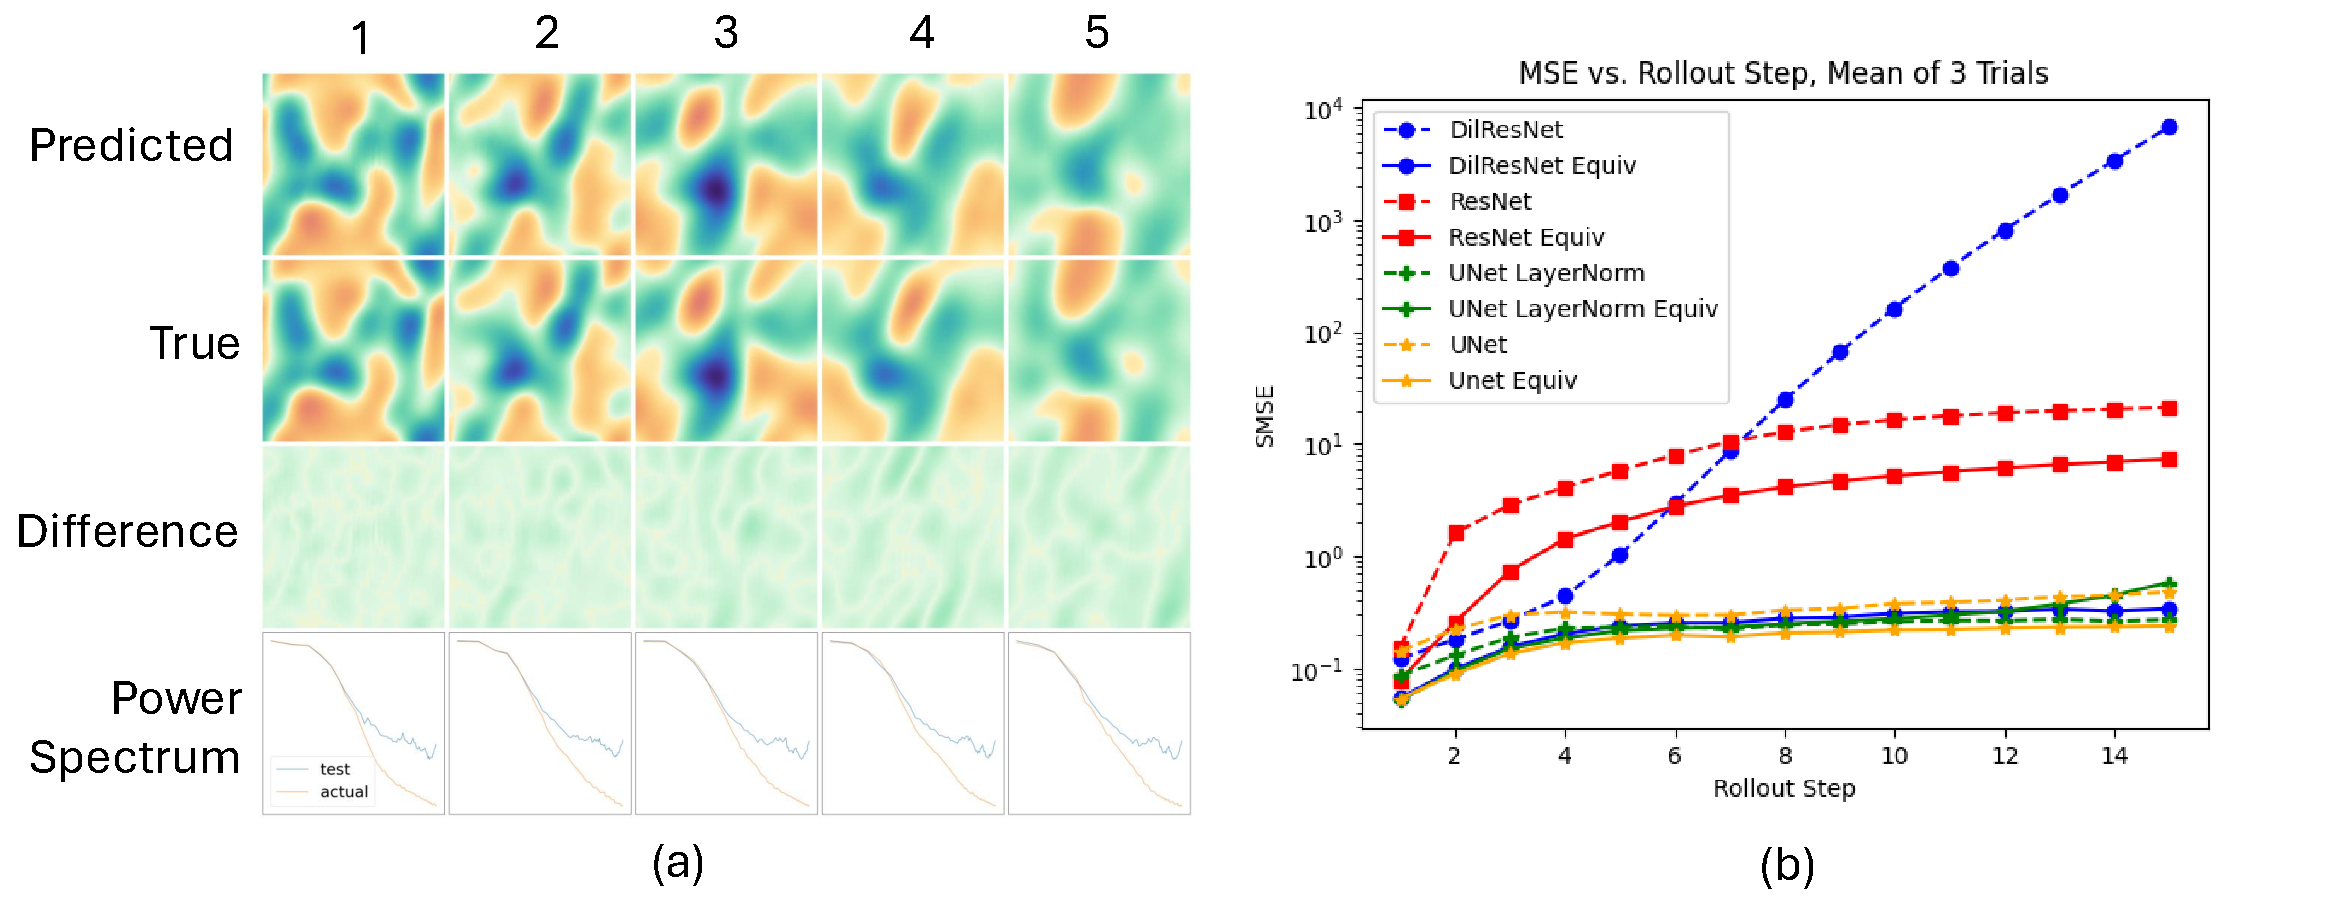
\includegraphics[width=\textwidth]{figures/cfd_results.pdf}
    \caption{(a) Five steps of rollout using the best performing model, the equivariant UNet without LayerNorm. 
    The x-component of the velocity is plotted.
    (b) Comparison of test performance over a 15 step rollout.
    The SMSE is shown for \textit{each} step, rather than a cumulative loss.}
    \label{fig:cfd_results}
\end{figure}

\paragraph{Hybrid methods}
Although emulators can be useful for quickly creating large amounts of simulations and can be used in downstream tasks, such as comparing with real data, the accuracy of the simulations produced will be fundamentally limited by the accuracy of the simulation used to train the emulator. Therefore, improving the quality of the simulation tool kits we have is as important as speeding up the simulation process with emulation. ML methods offers tremendous flexibility to learn complicated function, but this flexibility can sometime limit the maximum accuracy of a model. Therefore, combining ML methods with traditional PDE solvers has been a popular way to model dynamical systems when there is a strong requirement on the accuracy of the simulation \cite{Kidger2022OnND, Rackauckas2020UniversalDE}.

Instead of learning an end-to-end emulator of the simulation, in this task we aims to improve the accuracy of the simulations by replacing certain terms in eq. \ref{eq.QG2} with ML models. One way this can be achieved is through fitting some of the more uncertain term to observational data.
As a proof-of-principle step, we are first going aim to recover certain specific terms used to generate the data with ML models, that is to first generate a set of reference simulations, then try to recover some terms we deliberately leave out in the QG equation with ML methods. This will test the identifiability of the PDE model from data in practice. For example, $r_{ek}$ is a coefficient which is often assumed to be a fixed value. Instead, we can leave that as a free parameters and try to fit it with data. This process can also be applied to other more complicated terms in the equation (though we are aware that the inverse problem is not always solvable). We are also going to benchmark whether equivariant model outperforms its non-equivariant counterpart in recovering the missing term. Once we have validated the performance of our pipeline with our own simulation suite, we are going to improve our hybrid model by calibrating it to publicly available data \cite{2004AGUFMSF31A0712O}. 
As a result, this task will deliver a framework of ML-enhanced simulations designed for modeling ocean dynamics, which can be fitted to real data to capture unknown physics while maintaining the structure in eq. \ref{eq.QG1} that are stemmed from physical principle, such that it is capable to robustly generalize to systems that are significantly different from existing simulations. We will then be able to emulate enhanced hybrid models to create large ensembles for data assimilation.

\subsection{Thrust 2: Modeling real data with broken symmetries}

While Thrust 1 focuses on improving and speeding up simulations in an ideal situation, the focus of Thrust 2 will be on handling data that are not exactly equivariant. While the underlying physical phenomena in the real world obey symmetric physical laws, and therefore are exactly equivariant, the process of capturing or collecting data related to these physical phenomenons often breaks the exact equivariance. One example of this is ocean imaging, which introduces discretization to the underlying continuous physical phenomenon. 

Another case of broken symmetries is when a model excludes important quantities such that without them the model loses symmetry. For a toy example, think of a pendulum in 3D, the dynamics of the pendulum is coordinate-free; however, the pendulum dynamics is not a 3D-rotation-equivariant function of the position and velocity of the mass. This is because a change of coordinates will also rotate the gravity vector. In other words, the pendulum dynamics is a 3D-rotation-equivariant function of the position and velocity of the mass, and the gravitational acceleration (see, eg, \cite{villar2023passive}). In ocean dynamics, one example of this is the symmetry breaking caused by Earth rotation: A model that does not account for the relevant pseudo-scalar will look chiral.

In addition to discretization and modeling issues, it is inevitable for real life measurements to be contaminated by noise, which do not follow the same equivariance structure the interested process has. This means our data is not exactly equivariant, but instead contains signals that are exactly equivariant. In the simplest case, this process of taking data from an equivariant process can be defined as $\mathbf{d} = f(\mathbf{s}) + \mathbf{n}$, where $\mathbf{d}$ is the vector of data we obtain, $\mathbf{s}$ is the process that is equivariant, $f$ is a function that operates on $\mathbf{s}$ that could break the equivariance, e.g., discretization, and $\mathbf{n}$ is the random noise that is not equivariant.
Once the non-equivariant effects are introduced in the data, the data is no longer exactly equivariant but approximately equivariant.
The main questions that this Thrust aims to address can then be phrased as: given some data $\mathbf{d}$ that contains a signal that follows a particular equivariant structure, can we develop a method to extract the equivariant component from the data? Ultimately, we will not be able to perfectly extract the exactly equivariant signal from the approximately equivariant data, as that would require perfect characterization of the noise. So instead, the next best objective that is achievable is to bound the bias induced by the noise as much as possible. 

As the community begins to realize the importance of understanding approximate equivariance in order to apply equivariant models to real data, there have been some preliminary results in the literature \cite{Wang2022ApproximatelyEN, huang2021traffic}. For instance, in \cite{huang2024approximately} we mathematically study the bias-variance trade-offs of reducing the amounts of symmetries that a model implements. 
In this Thrust, we build on top of the infrastructure prepared in Thrust 1, but shift our focus to adding effects to understand the behavior of equivariance models when presented approximately equivariant data. This Thrust contains two complementary directions  

\paragraph{Understanding the scale of equivariant signals}
In the example from \cite{gregory2024robust} illustrated in Figure \ref{fig:cfd_results} we used a GeometricImageNet which is an architecture similar to the convolutional neural network (CNN) but with imposed equivariance to emulate simulations of 2D compressible Navier-Stokes equation. 
Once we trained the network in a supervised setting, we also inspected how the network would perform in ``roll-outs", i.e. integrating the trajectories from an initial condition using the network as a forward step. This is usually a good measure of whether the training is robustly capturing the physics or just overfitting to the data.

One of the major surprises we found in this study was that by introducing dilation to a ResNet architecture \cite{yu2017dilated}, that is, by introducing gaps between elements in the convolution kernels, we improved the rollout accuracy by a factor of $\sim 20$ while reducing the number of parameters by a factor of 2. On the other hand, we repeated the experiment with the corresponding non-equivariant baselines, and the results of the dilated ResNet were catastrophic: it was three orders of magnitude worse than the non-dilated version. This result suggests that the equivariant neural networks can pick up signals from specific scales, hence drastically improve the generalization accuracy. In many analyses related to physics systems, the accuracy of analysis improves when the scale of tools matches the scale of the dynamics.

In this task, we aim to mathematically and empirically analyze the joint effects of equivariance and scale.
We are going to investigate the role scale plays in training an equivariant neural network and aim to come up with a concrete formalization of the response of equivariant neural network to data as a function of scale under discretization. Ideas of this sort have previously appeared in the numerical analysis literature, showing that numerical methods based on discretizations that respect the symmetries of the underlying problems outperform ones that do not \cite{verstappen2003symmetry}.  The empirical study will be done with training data from the 2-layer QG ocean model as described in eq\ref{eq.QG1}, for which we have control over the scales of features. The next step is to train a collection of equivariant neural networks on the generated data, while varying the scale of the kernel used in the network, to investigate the dependence of the kernel size on the equivariant scale.

\paragraph{Disentangling equivariant processes from noise}
Another difference between theoretical data and real data is the presence of noise \cite{Wang2022ApproximatelyEN}. Since noise is not expected to be equivariant, adding noise to any equivariant signal will break the symmetry. Noise could originate from multiple types of sources at different scales. To illustrate this, let's use taking a satellite picture of the ocean as an example: at the pixel scale, there will be instrument noise from the camera that introduce fluctuation in the pixel reading; at the largest scale, there will be processes that irrelevant to the objectives such as cloud occlusion. 

The concrete definition of the problem in this task is: Given some noisy observation of a process that exhibits some equivariance, can we disentangle the information related to the equivariant process from the noise in an unsupervised manner?

As a starting step, we will use the simulations generated in Thrust 1 as the base, then we are going to add different realizations of noise to the simulations to create signals that are not exactly equivariant.  We will repeat the experiment in task 1, except now we introduce a simple yet controllable Gaussian noise process following a specific power spectrum. In this way, we can control whether the noise is more prominent in smaller scales or larger scales. 

\subsection{Thrust 3: Adversarial attacks and robustness}
% HOGG: Reference: Perezhogin et al \url{https://arxiv.org/pdf/2302.07984.pdf}

While Thrust 2 investigates how bias is introduced steadily via noise, this Thrust looks into how bias can be introduced so drastically that it creates catastrophic failures, and how to defend against such catastrophic failures.
When simulating a particular PDE, errors accumulate as we integrate forward in time.
Traditional PDE solvers have guarantees on how rapidly the error can grow, often related to the order of the solver. For example, the Euler method has global error that grows linearly.  However, there are no such guarantees for ML based methods. Most of the uncertainty quantification approaches are based on estimating the bias and the variance of the predictions via Bayesian approaches or other machine learning models \cite{perezhogin2023generative}.

%As we mentioned in Thrust 2, this lack of guarantee is not only  unsettling from a rigor point of review, the practical reason to avoid using methods without such guarantee is to avoid potential catastrophic failures.
As we have shown in \cite{gregory2024robust}, catastrophic failures did occur when using a dilated ResNet to model a compressible Navier-Stokes equation. Another form of catastrophic failures these models may be susceptible to are adversarial attacks.


Adversarial attacks are an interesting phenomenon that was identified in large machine learning models \cite{goodfellow2014explaining} about ten years ago. In many high-accuracy machine learning models, a small, carefully crafted perturbation to the input data can drastically change the output of the method. One of the classic examples of an adversarial attack is the single-pixel attack \cite{su2019one}, in which one only needs to change the value of one-pixel of the input image to alter the result of a classification task.

In the context of ocean simulations, the question of interest is whether similar small perturbation can lead to a drastic non-physical deviation in the dynamics. This is especially important when rolling out a learned emulator to an ocean model, since noise can accumulate and interact with the simulation non-linearly.

Compared to standard ML methods, equivariant models have more constraints in their architecture. It is possible that at least certain kinds of attacks are likely to be less effective or not effective at all.  There exists some literature on adversarial attacks of equivariant models \cite{schuchardt2023provable}, but similar to approximate equivariant models, the literature in adversarial attacks in the context of equivariant model is still underdeveloped. 

In this Thrust, we will explore how to empirically avoid catastrophic failures when applying ML methods to ocean simulations in two steps: First we will create experiments to adversarially attack equivariant models. The goal of this task is to understand the adversarial robustness of the proposed models empirically. The second step in this Thrust is to build methods that are robust against such attacks, possibly following ideas from \cite{schuchardt2023provable}.

\section{Future Naval Relevance}
The priorities of this proposal call are \hogg{I will write words here about the CFP and our connection to the keywords there. Also: Navy needs to understand oceans!}

\section{Project schedule and milestones}\label{sec:deliverables}

The deliverables of this three-Thrust project will be:
\begin{enumerate}
    \item A theoretical understanding on what role symmetry plays in modeling complex physical system with ML, specifically when used together with a physics-driven model.
    \item The library of simulations generated will be made available to the public. This provides the community with a domain-specific benchmark dataset.
    \item Our code will be open-source (and published on GitHub). The tightly integrated machine-learning--physical model can be a blueprint for other researchers to build on.
    \item Machine learning models for emulation of ocean dynamics and closures that are equivariant and robust to adversarial attacks. HOGG FIX THIS.
    \item Activities such as curating a well-put-together library can create a lot of research opportunities for junior researchers such as undergraduate and graduate research assistants. On one hand, the domain-specific knowledge from Zanna's group hones the student's understanding of the physical model. On the other hand, the students are also exposed to state-of-the-art ML applications. This project will help train next-generation scientists specialized in ocean dynamics who are well-versed in both physical modeling and ML.
    \item Every significant result from this project will be written up in papers for the peer-reviewed literature in mathematics, ML, or ocean science, as appropriate. When relevant, papers will be submitted to the large ML conferences or the workshops thereof. 
    \item HOGG: IS THIS LIST COMPLETE? 
\end{enumerate}
The timeline for the project is shown in Figure~\ref{fig:timeline}.

\begin{figure}
    \centering
    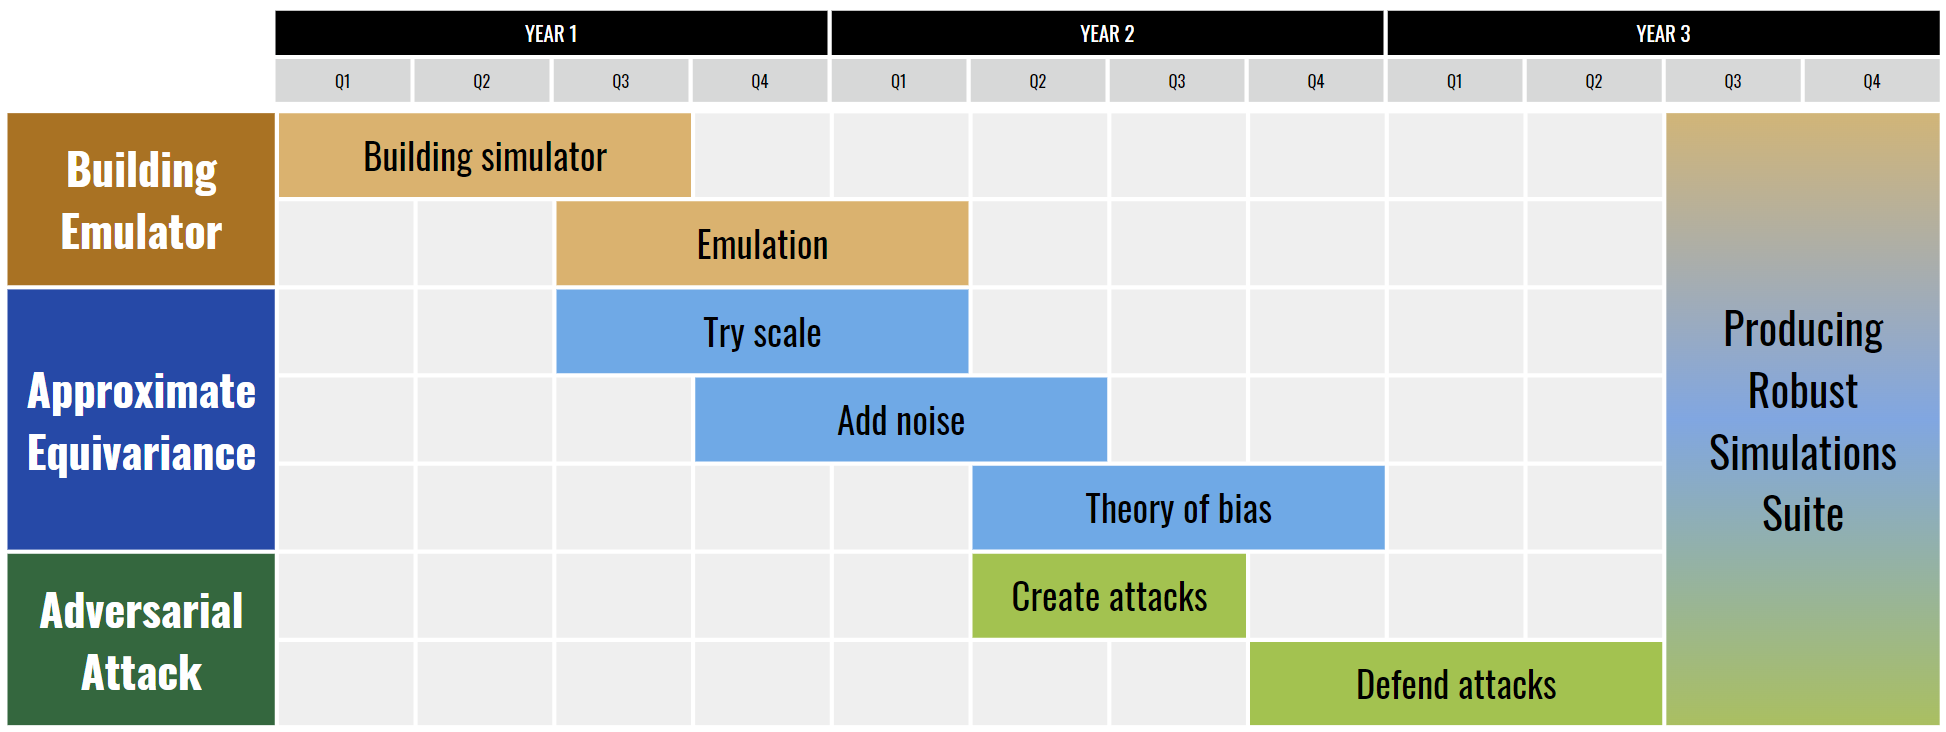
\includegraphics[width=0.9\linewidth]{figures/ONR_gnatt_chart.png}
    \caption{Timeline for the project activities, organized by Thrust.}
    \label{fig:timeline}
\end{figure}

\section{Management Approach}
This proposal comes to ONR in the form of a pair of related proposals from New York University and Johns Hopkins University.
There are therefore two budgets, one at NYU, divided between the Department of Physics and the Courant Institute of Mathematics, and one at JHU in the Applied Mathematics and Statistics Department.
The NYU budget will support two 12-month graduate student researchers, one in the Physics Department and one in the Courant Institute.
The JHU budget will give partial salary to research professor Kaze Wong, and support a part-time undergraduate researcher.
In addition, the three PIs will each receive a small amount of summer salary support.

The NYU and JHU groups already work together well, with semi-regular meetings to discuss interfaces between mathematics, machine learning, differential equations, and ocean physics.
With the formalization of this project as an ONR-supported effort, we will schedule weekly videoconferences between JHU and NYU to keep all project personnel working together and up-to-date on progress and challenges.
In addition, we will schedule an annual two-day meeting of all personnel in Baltimore, and an annual two-day meeting of all personnel in New York.
There is some funding budgeted for these collaboration meetings.

Because the three PIs work well together, the plan is to work collaboratively on all project sub-parts.
There are enough deliverables and results to ensure that junior personnel will have projects to individually lead, while contributing to all components.

In addition, we have budgeted for some travel by the project participants to domestic and international conferences.
We have not budgeted for hardware, because all computing needs for this project can be met with the high-performance computing facilities at NYU and JHU.
% HOGG MAKE SURE THIS IS ALL TRUE.

\section{Principal Invesgitator Qualifications}

There are two PIs at NYU---David W. Hogg and Laure Zanna---and one at JHU---Soledad Villar.

\paragraph{David W. Hogg}
Interested in precision measurement, primarily in astrophysics-related domains, PI Hogg is a leader in developing new data analysis methodologies and systems for the physical sciences.
He has been the PI of XXX Federal Grants, XXX from NASA and YYY from NSF, for a combined total of XXX USD.
In addition, he was co-PI on a \$35M grant from the Moore and Sloan Foundations to create a Data Science Environment across three US universities.
He has ample experience managing external funding of the kind proposed here.

Hogg has been involved in developing open-source software tools for astrophysics, including the emcee package (CITE) for adaptive monte-carlo integration of probability models, and the Astrometry.net package (CITE) for automated recognition and calibration of astronomical imaging.
The former of these (emcee) has 13,000 citations, mostly in physical-sciences domains.
His group in New York supports more than a dozen open-source software packages with users and active development communities.
The methods, code, and software developed in this proposal will be managed well, as with his previous projects.

Along with open-source code, Hogg supports open science by helping to design, build, operate, and manage large astronomical projects that produce open data products.
He has been involved in all five phases of the Sloan Digital Sky Surveys, since 1998, and has been a co-author on all 19 data-release publications therefrom.
Currently he serves as the Chair of the Advisory Council for SDSS-V; this body represents the interests of the 70 academic partners involved in the project.
He is also on the Board of the Terra Hunting Experiment, a new project to build and operate a robotic spectrograph--telescope system at the Isaac Newton Telescope.

Hogg has directly supervised 13 PhD students through to graduation, and has 4 current students.
He has supervised more than 20 postdoctoral scholars, at NYU and the Simons Foundation.
Although Hogg has a role in the Simons Foundation, he recieves no direct cost support for his students or research program from the Foundation; he raises all his funding for PhD students externally to NYU and externally to the Simons Foundation.

Recently, Hogg (with PI Villar) has developed new methods for machine learning that incorporate the exact physical symmetries of permutation, translation, rotation, and boost covariances (CITE), and even the symmetry of units covariance (dimensional analysis; CITE).
These methods work well in many physical domains, and these projects inspired the current proposal.

\paragraph{Soledad Villar} \hogg{Sole: Please put in text here.}

\paragraph{Laure Zanna} \hogg{Laure: Please put in text here.}

\section{Responsibility}
\hogg{Describe how you have adequate resources
or the ability to obtain such resources as
required to complete the activities proposed.

Describe how you have the ability to comply
with the grant conditions, taking into account
all existing and currently prospective
commitments of the applicant,
nongovernmental and governmental.

Describe your performance history;
specifically, your record in managing
Federal awards and the extent to which any
previously awarded amounts will be
expended prior to future awards.

Describe your record of integrity and
business ethics.

Describe qualifications and eligibility to
receive an award under applicable laws and
regulations.

Describe your organization, experience,
accounting, and operational controls and
technical skills or the ability to obtain them
(including as appropriate such elements as
property control systems, quality assurance
measures, and safety programs applicable to
the efforts to be performed).}

\section{Data Management Plan}
\hogg{In no more than 2 pages, discuss the following:

The types of data, software, and other
materials to be produced.
`
How the data will be acquired.

Time and location of data acquisition, if
scientifically pertinent.

How the data will be processed.

The file formats and the naming conventions
that will be used.

A description of the quality assurance and
quality control measures during collection,
analysis, and processing.

A description of dataset origin when existing
data resources are used.

A description of the standards to be used for
data and metadata format and content.

Appropriate timeframe for preservation.

The plan may consider the balance between
the relative value of data preservation and
other factors such as the associated cost and
administrative burden. The plan will provide
a justification for such decisions.}

\clearpage
\section*{Bibliography and References Cited}
\bibliographystyle{IEEEtran}
\renewcommand{\bibsection}{}
\bibliography{emulator}

\clearpage
\section*{Facilities and Other Resources}
\hogg{This needs to be different between the NYU and JHU proposals. I think we can handle this with input files in latex.}

The NYU Department of Physics is part of the NYU Faculty of Arts \& Science and includes the Center for Cosmology and Particle Physics (the home of PI Hogg), the Center for Soft Matter Research, and the Center for Quantum Phenomena.
The NYU Department of Mathematics is part of the Courant Institute and includes the Center for Atmosphere Ocean Science (the home of PI Zanna).
A wide variety of sponsored
research activities take place in both Departments.
These range from
the theoretical to the pragmatic, and include a broad spectrum of
interactions with such disciplines as astronomy, biology, medicine, chemistry, and computer science.

In addition to benefiting from this research activity directly and indirectly, as members of these Departments, the PIs receive through their home Departments staff support for clerical work, post-award grant support, and for computing (expanded upon below).

\paragraph{Computing Equipment at Physics:}
The astrophysics group at NYU maintains some high-performance computers
for the PI, and substantial storage machines.
The latter contain more than 100~Tb of disk space, most of which is filled
with astrophysical imaging data.  The Physics Department maintains a
state-of-the-art controlled-environment computer room.

The University has hired a Director of Scientific Computing for the
NYU Center for Cosmology and Particle Physics.  His
responsibilities include management of the cluster and the data
servers, and overall management and supervision of the Center's
computer system.  He will oversee the computer hardware used in this
project.

A variety of computing resources are available within the Physics
Department, including UNIX workstations, laptops, laser color
printers, etc.  The Department runs a network of several hundred
desktop workstations, file servers, in addition to the multi-processor
computational server mentioned above.

\paragraph{Computing Equipment in Courant:}
\hogg{LZ: Details about computing inside Courant?}

\paragraph{Other NYU Computing Resources:}
Computational needs are also supported through the University's
Academic Computing Services, a unit of the NYU-wide Information
Technology Services offering an additional wide range of computational
resources in support of research and instruction.  These include a
variety of computing platforms, including several high-performance
multi-CPU and multi-GPU systems, and scientific software.  Consultants are available
to assist in the use of these resources.

Finally, the NYU Center for Data Science (where PI Hogg is affiliated)
maintains some specialized high-performance machines for machine-learning
applications, some of which are relevant to the proposed project.

\paragraph{Office Space:}

The offices of the personnel will all be located in the NYU Physics and Mathematics Departments.

In addition, through the NYU Center for Data Science, PI Hogg has access to temporary studio space, work space, visitor space, and meeting space.

\paragraph{Library Resources:}

In addition to an enormous book collection, the NYU libraries hold
current subscriptions to hundreds of hardcopy and electronic journals.
It provides access to all journals relevant to this project and such
databases as MathSciNet, the Web of Science (science citation index),
and the ACM Digital Library.

\paragraph{Experimental and Hardware Facilities:}

Both the Physics Department and Math Department have experimental facilities, including machining, imaging, and clean facilities, but none of these are directly relevant to this project, except insofar as they are part of the rich intellectual and research atmosphere.


\end{document}